\documentclass[main.tex]{subfiles} 
\begin{document}

\section{VIDEO COMPREHENSION SCORE (VCS): A METRIC FOR LONG-FORM VIDEO DESCRIPTION EVALUATION}

\subsection{INTRODUCTION}

Recent advancements in Large Video Language Models (LVLMs) \cite{Yuan2025Tarsier2,Shen2025LongVU,Ataallah2024Goldfish,Chen2025LongVILA} have enhanced automated video comprehension, enabling long-form description generation from long videos. However, exploratory analysis on long videos reveals that LVLMs frequently (i) miss global narrative structure, (ii) fail to capture local events, and (iii) fail to establish temporal connections while hallucinating content. These gaps indicate LVLMs lack true video comprehension, raising the question: how can we evaluate models' video comprehension? Current benchmarks utilize question-answering formats \cite{wu2024longvideobench,ataallah2024infinibench,nagrani2025neptune} or short-form description comparisons for short videos \cite{wyzs:24,chen:acl11,ZhXuCoAAAI18}, both inadequate to evaluate models' true video comprehension ability. Evaluating genuine comprehension demands shifting to a methodology that processes long or complex videos and requires models to generate long-form descriptions. This approach renders superficial frame-level analysis insufficient, compelling models to instead generate outputs that capture global narrative structure, detail specific local events, and establish their temporal relationships. The quality of these generated descriptions can then be evaluated against the source video or human-written descriptions.

Description-based evaluation methods fall into four categories, each struggling with fundamental aspects of long-form evaluation. N-gram metrics such as BLEU \cite{p:02}, METEOR \cite{bl:05}, CIDEr \cite{v:15}, and ROUGE \cite{l:04} rely on lexical overlap, which not only unfairly penalizes legitimate paraphrases but also rewards superficial word-level matches between descriptions with entirely different global narratives. Embedding-based metrics like BERTScore \cite{z:20} and SBERT \cite{r:19} address lexical limitations through semantic similarity but overlook chronological alignment and local fine-grained details, allowing misordered events and subtle errors to remain undetected. Multimodal metrics such as EMScore \cite{syxl:22} enable direct comparison against source video content but struggle with long videos and long-form descriptions. LLM-based metrics such as CLAIR \cite{chan:23} and AutoDQ \cite{wyzs:24} provide deeper insights but often do not evaluate the chronology of events while suffering from consistency issues.

To address these limitations, we introduce VCS with three components:
\begin{enumerate}
\item \textbf{Global Alignment Score (GAS)}: Measures global thematic alignment.
\item \textbf{Local Alignment Score (LAS)}: Assesses local semantic alignment.
\item \textbf{Narrative Alignment Score (NAS)}: Evaluates chronological alignment using configurable Local Narrative Tolerance (LNT).
\end{enumerate}

VCS combines these three components to provide comprehensive evaluation: GAS and LAS form the Semantic Alignment Score (SAS), which integrates with NAS to produce the final VCS score. We also present VCS$_{\text{short}}$, which applies the same framework to short-form descriptions.

To evaluate VCS, we need datasets of long-form video descriptions paired with quality assessments—but no such datasets exist. Although creating a human-annotated dataset with quality ratings would be ideal, it is impractical: producing and reviewing long-form descriptions is costly and time-consuming, and annotator agreement declines sharply as description length increases. We therefore constructed a large-scale synthetic dataset from the MPII Movie Description Dataset \cite{rohrbach2015dataset} via ChatGPT-4o. From this dataset, we derived two test sets: a Corruption Detection Test Set to evaluate VCS ability to distinguish valid variations from invalid corruptions, and a Cross-Author Consistency Test Set to assess robustness across different authorial styles. VCS consistently outperforms traditional metrics on corruption detection tasks. To assess human correlation, we evaluate VCS$_{\text{short}}$ on VATEX-EVAL \cite{syxl:22}, where it achieves state-of-the-art results. These results demonstrate VCS effectiveness for robust evaluation of both long-form and short-form video descriptions.

Our primary contributions include:
\begin{itemize}
\item A robust metric (VCS) for both long-form and short-form video descriptions.
\item Configurable LNT and chunk size parameters to govern chronological strictness and comparison granularity.
\end{itemize}

\subsection{RELATED WORK}

Traditional n-gram-based metrics such as BLEU \cite{p:02}, ROUGE \cite{l:04}, and METEOR \cite{bl:05} evaluate text generation through lexical overlap and local word order. BLEU measures n-gram precision with brevity penalties, capturing local ordering but missing event-level chronology and struggling with expressive variability. ROUGE variants compute precision, recall, and F1-scores: ROUGE-N evaluates n-gram overlap, ROUGE-L computes Longest Common Subsequence at summary-level, and ROUGE-Lsum calculates sentence-level LCS by splitting at newlines. While preserving sequential information, they miss event-level chronology and remain sensitive to expressive variability. METEOR addresses expressive variability via synonyms and stems, computing recall-weighted F-scores with fragmentation penalties, but similarly misses event-level chronology. CIDEr \cite{v:15} uses consensus-based TF-IDF weighting across multiple references but proves impractical for long-form descriptions due to labor-intensive annotation. SPICE \cite{afjg:16} evaluates semantic propositions using graph overlaps, effectively handling paraphrasing; however, being designed for static images, it cannot be directly applied to videos and neglects narrative chronology critical for video descriptions.

Embedding-based metrics compare texts in semantic vector spaces, leveraging pretrained models to capture semantic similarity beyond lexical matches. BERTScore computes token-level similarity using contextualized BERT embeddings, aggregating optimal alignments into precision, recall, and F1-scores, while SBERT employs siamese networks with mean-pooling for sentence-level embeddings, but both address expressive variability by recognizing paraphrases yet are constrained by limited context windows, complicating their direct application to long-form descriptions. Recent decoder-based models such as NV-Embed-v2 \cite{l:24}, Linq-Embed-Mistral, SFR-Embedding-Mistral, and Jasper and Stella leverage autoregressive LLM architectures with bidirectional attention, offering significantly larger context windows and robust global embeddings, excelling at paragraph-level semantic assessments. However, reliance on global embeddings and cosine similarity overlooks local content alignment, detailed information accuracy, and chronological alignment.

Multimodal embedding metrics like EMScore \cite{syxl:22} and PAC-S employ vision-language models such as CLIP \cite{Radford2021LearningTV} to evaluate semantic alignment between visuals and generated captions, addressing expressive variability through direct image-caption comparison, thus bypassing reference captions. EMScore computes video-caption similarity through dual-level matching: coarse-grained alignment between video and caption embeddings, and fine-grained matching between frames and words, calculating precision, recall, and F1-scores via cosine similarity. PAC-S fine-tunes CLIP through positive-augmented contrastive learning with synthetic image-text pairs, then computes cosine similarity scores from the enhanced model. Despite their effectiveness in short-form descriptions, these metrics face computational challenges and methodological limitations when scaling to long-form descriptions.

Recent evaluation approaches increasingly leverage Large Language Models (LLMs), categorized into component-based and holistic judge methods. Component-based methods such as AutoDQ \cite{wyzs:24} extract events from descriptions using ChatGPT, then compute precision and recall through entailment analysis comparing extracted events between texts, while VAD-Score employs LLMs for semantic extraction and scoring of events, subjects, and objects, effectively addressing expressive variability but missing chronological evaluation. Holistic methods such as CapScore prompt GPT-4 to score caption similarity and quality, CapArena-Auto Score uses GPT-4o for pairwise evaluation battles, and CLAIR \cite{chan:23} employs zero-shot prompting for similarity scores with interpretable reasoning. However, these methods suffer from ambiguity in score calibration, sensitivity to prompting nuances, consistency issues across model versions, limited interpretability, and practical constraints including reproducibility and cost.

\subsection{METHODOLOGY}
\label{sec:methodology_vcs}

Figure~\ref{fig:vcs-architecture} shows the VCS pipeline, which computes semantic and narrative alignment between reference and generated descriptions to achieve comprehensive long-form video description evaluation.

\begin{figure*}[t]
\centering
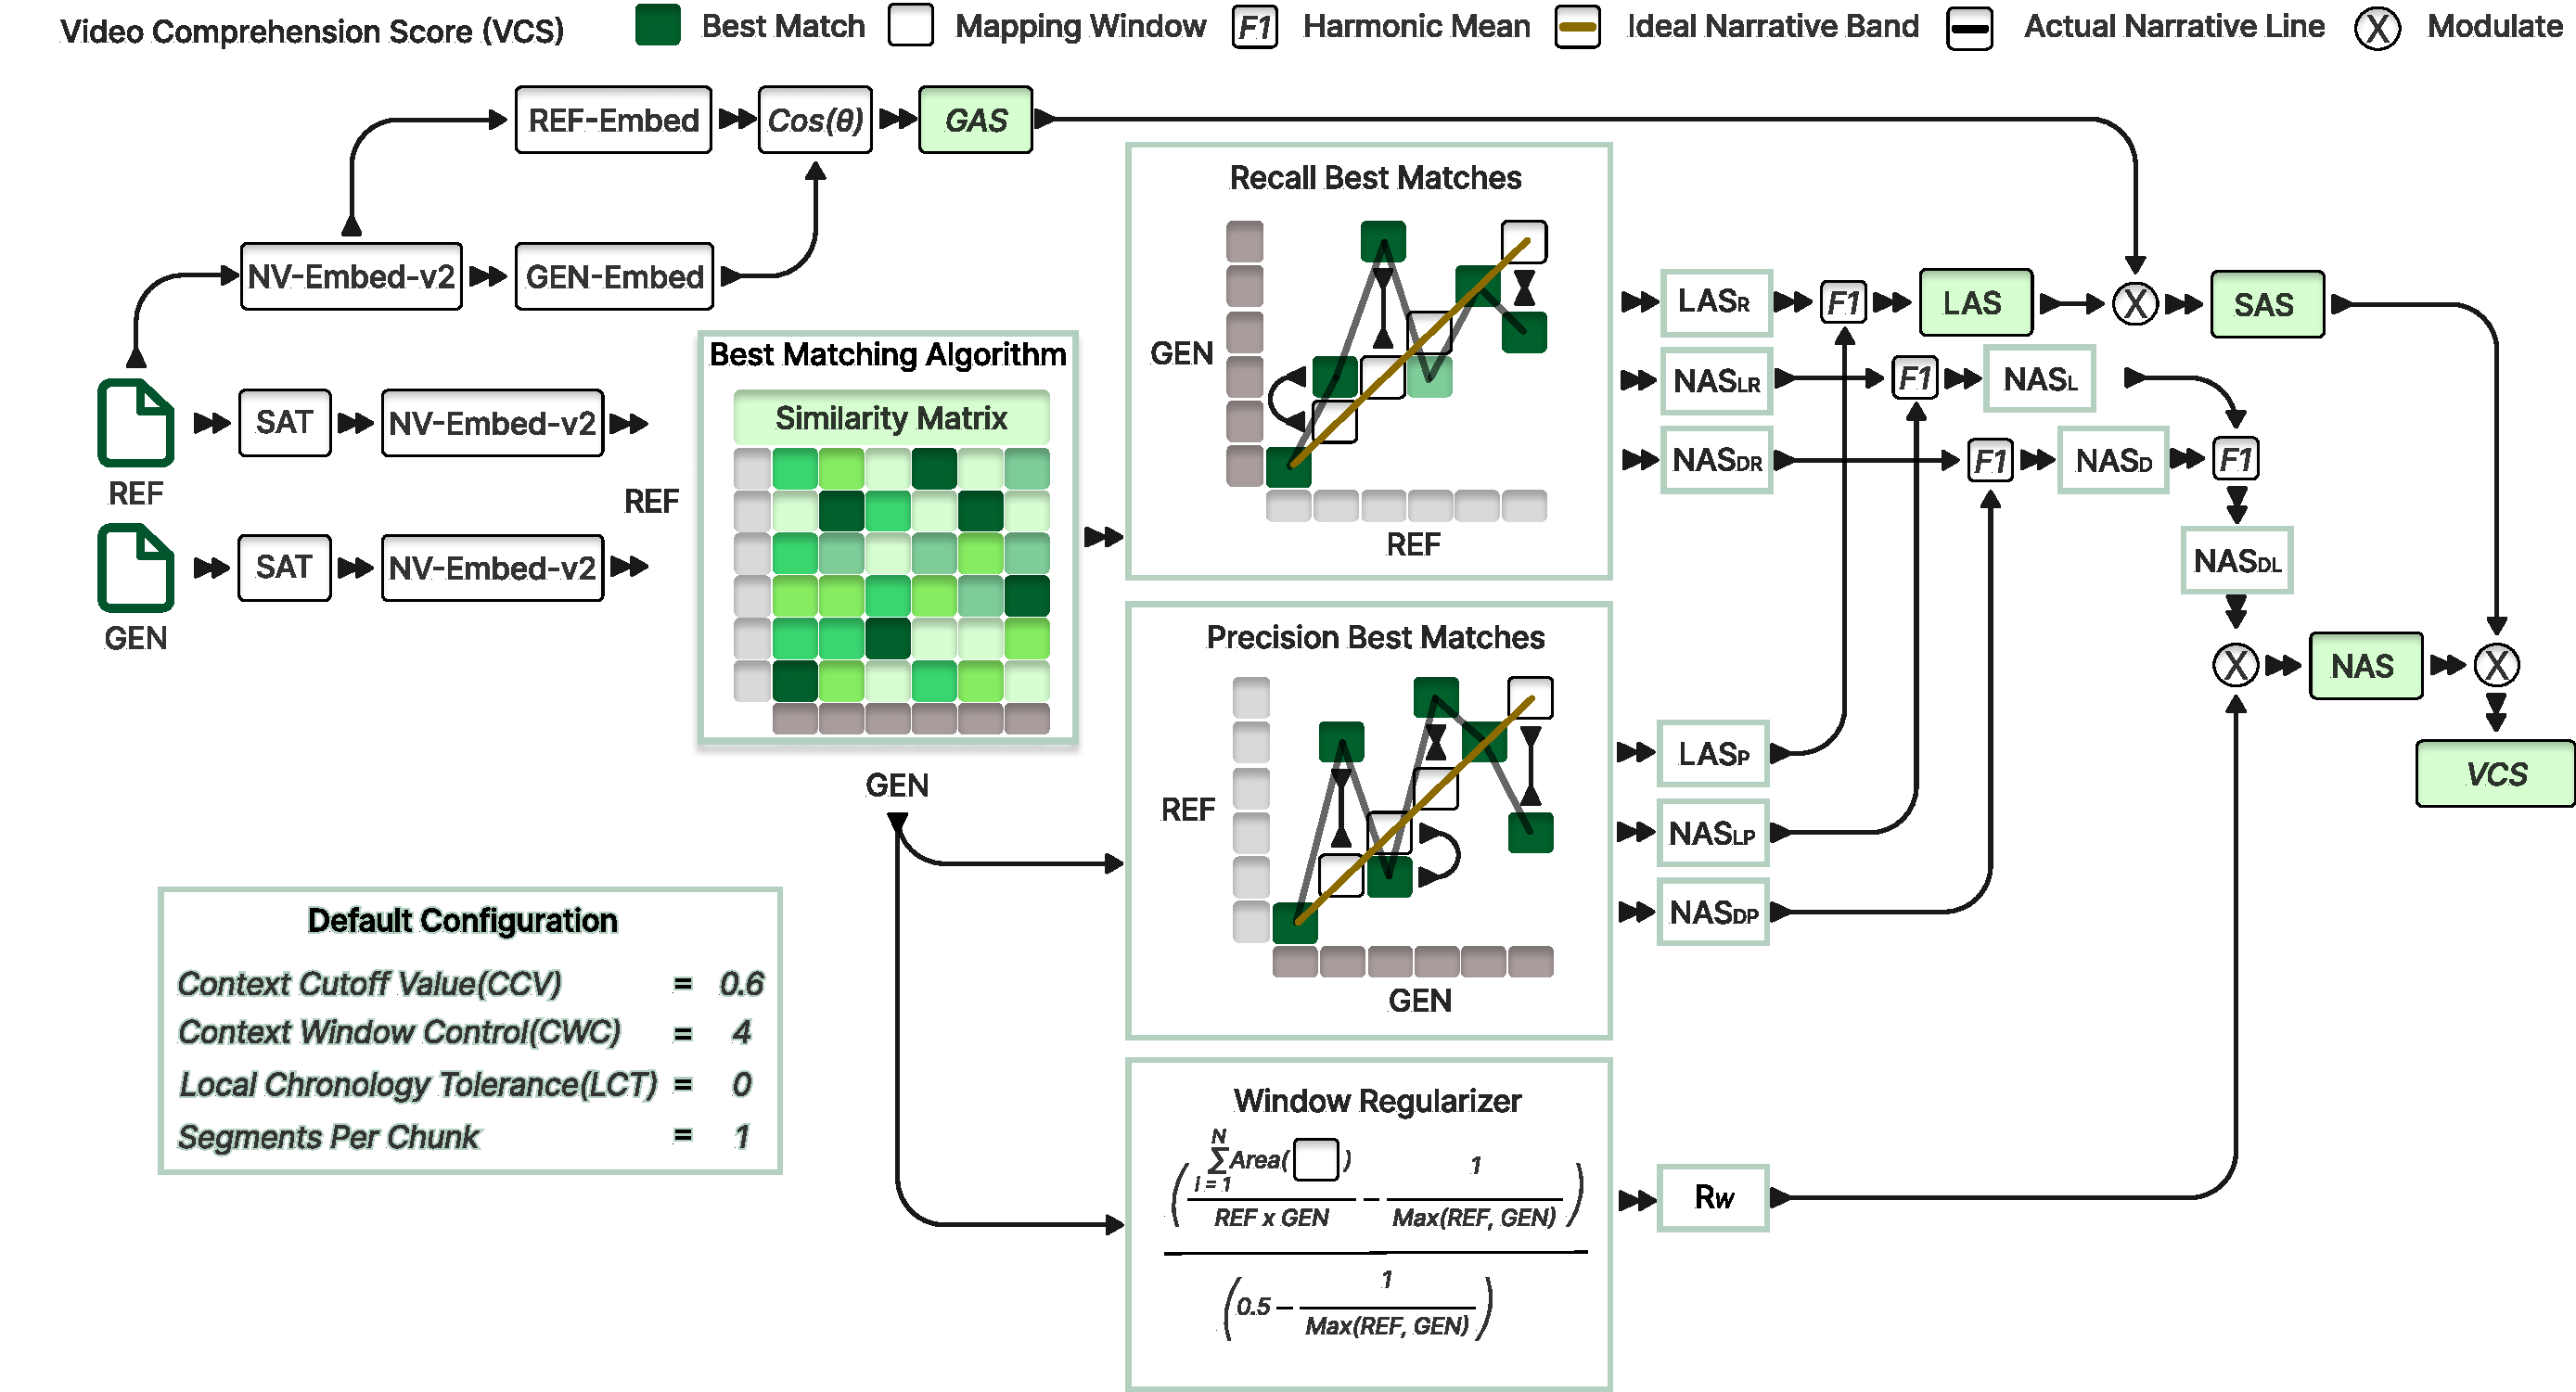
\includegraphics[width=0.8\textwidth]{images/VCS.pdf}
\caption{VCS Pipeline. The VCS assesses video descriptions by comparing a reference text ($T_{ref}$) with a model-generated text ($T_{gen}$). Both texts are initially segmented by SaT and embedded via NV-Embed-v2. The Global Alignment Score (GAS) is computed from the full text embeddings. For localized analysis, texts are chunked and embedded, forming a similarity matrix. From this, precision and recall-oriented best matches yield the Local Alignment Score (LAS)—the harmonic mean of $LAS_P$ (precision) and $LAS_R$ (recall). The Narrative Alignment Score (NAS) incorporates distance-based ($NAS_D$) and line-based ($NAS_L$) assessments. $NAS_D$ and $NAS_L$ are harmonic means of their respective P and R components. A Window Regularizer ($R_w$) refines the NAS. The Semantic Alignment Score (SAS) combines GAS and LAS through two-stage semantic assessment. The final VCS integrates SAS with the regularized NAS where the weaker component regularizes the stronger one.}
\label{fig:vcs-architecture}
\end{figure*}

\subsubsection{Global Alignment Score (GAS)}
VCS computes GAS to capture global thematic alignment between reference and generated descriptions. Given input texts $T_{ref}$ and $T_{gen}$, we encode each description using NV-Embed-v2. The GAS is computed as:

\begin{equation} \label{eq:gas_revised}
\text{GAS} = \frac{\mathbf{E}_{ref} \cdot \mathbf{E}_{gen}}{\|\mathbf{E}_{ref}\| \|\mathbf{E}_{gen}\|}
\end{equation}

\subsubsection{Text Preprocessing for Chunk-Level Analysis}
However, GAS lacks sensitivity to fine-grained details and chronological consistency. To enable fine-grained analysis, VCS applies punctuation removal and Segment Any Text (SaT)~\cite{frohmann-etal-2024-segment} segmentation to $T_{ref}$ and $T_{gen}$, producing semantic segments $S_{ref}$ and $S_{gen}$. We group $k$ consecutive segments into chunks:
\begin{align}
C_{ref} &= \{c_1^{ref}, \ldots, c_{N_{ref}}^{ref}\} \\
C_{gen} &= \{c_1^{gen}, \ldots, c_{N_{gen}}^{gen}\}
\end{align}
embedded using NV-Embed-v2 to yield matrices $\mathbf{E}_{C_{ref}} \in \mathbb{R}^{N_{ref} \times D}$ and $\mathbf{E}_{C_{gen}} \in \mathbb{R}^{N_{gen} \times D}$.

\subsubsection{Defining Mapping Windows}
Before establishing chunk correspondences for fine-grained assessment, VCS constructs a similarity matrix to enable optimal alignments. Using $\mathbf{E}_{C_{ref}}$ and $\mathbf{E}_{C_{gen}}$, we compute similarity matrix:
\begin{equation}
\mathbf{S} \in \mathbb{R}^{N_{ref} \times N_{gen}} \text{ where } S_{i,j} = \cos(\mathbf{E}_{C_{ref}}[i], \mathbf{E}_{C_{gen}}[j])
\end{equation}
which represents the cosine similarity between the $i$-th reference chunk and $j$-th generated chunk.

VCS defines Mapping Windows (MW) that constrain the search space within this similarity matrix based on diagonal alignment patterns observed in ideal narratives.

VCS identifies the longer sequence as $\max(N_{ref}, N_{gen})$ and the shorter sequence as $\min(N_{ref}, N_{gen})$. We compute slope $s = \text{longer}/\text{shorter}$ and base window height $h_{mw} = \lceil s \rceil$, which represents the minimum height needed for each mapping window to ensure complete coverage of the timeline ratio. The algorithm creates direct windows by mapping each position $i$ in the shorter sequence to a window of height $h_{mw}$ in the longer sequence, spanning range $[\lfloor i \cdot s \rfloor, \min(\lfloor i \cdot s \rfloor + h_{mw}, \text{longer}))$ with proportional scaling. Reverse windows invert this mapping: for each position in the longer sequence, we determine which positions in the shorter sequence include it. VCS assigns Precision Windows ($MW_p$) and Recall Windows ($MW_r$) based on sequence direction: when $N_{ref} \geq N_{gen}$, precision uses direct windows and recall uses reverse windows; otherwise, assignments are reversed.

We define $MW_p = \{[s_i, e_i)\}$ as the set of precision Mapping Windows and $MW_r = \{[s_j, e_j)\}$ as the set of recall Mapping Windows, where each window $[s_k, e_k)$ represents the half-open interval from start index $s_k$ (inclusive) to end index $e_k$ (exclusive) of the $k$-th mapping window.

\subsubsection{Best Matching Algorithm}
Having established Mapping Windows within the similarity matrix $\mathbf{S}$, VCS pairs each generated chunk with its best reference counterpart, and vice versa. Naively selecting the highest-similarity reference for each generated chunk leads to semantic collision and semantic ambiguity. Semantic collision occurs when a single chunk exhibits identical similarity to multiple counterparts, while semantic ambiguity arises when a chunk achieves nearly equal similarity with multiple candidates. Both issues stem from repeated events or superficial lexical overlap, obscuring true narrative counterparts.

VCS resolves these issues through a Best-Matching Algorithm that combines adaptive context filtering with mapping-window constraints. Adaptive context filtering first determines a candidate set around the maximum similarity rather than committing immediately to the top score. Two user-defined parameters control this process: the context cutoff $\tau_{ctx}$ (default 0.6) and the context window control $k_{ctx}$ (default 4). Similarities below the cutoff receive no context expansion, while those above it define a context window whose width is computed as

\begin{equation}
w_{ctx} = \frac{(1-\tau_{ctx})-(1-s_{max})}{s_{max} \cdot k_{ctx}},
\end{equation}

where $s_{max}$ is the maximum similarity for the chunk. All candidates within $s_{max} - w_{ctx}$ enter the pool for selection. Mapping-window constraints then enforce temporal alignment: among the candidate matches, the algorithm chooses the chunk closest to the mapping-window boundary of the target chunk, breaking ties by similarity. When $s_{max}$ falls below the cutoff, no context expansion occurs, and ties are resolved purely by distance from the mapping-window boundary.

This combination mitigates both collision and ambiguity. Executing this procedure for each generated chunk and each reference chunk yields:
\begin{align}
M_P &= \{(C_j^{gen}, C_{i^*}^{ref})\} \quad \text{(precision best matches)} \\
M_R &= \{(C_i^{ref}, C_{j^*}^{gen})\} \quad \text{(recall best matches)}
\end{align}

\textbf{Pipeline Flow}: These correspondence sets $M_P$ and $M_R$ serve as the foundation for all subsequent VCS components. While the similarity matrix $\mathbf{S}$ contains comprehensive pairwise relationships, the Best Matching Algorithm distills this information into optimized correspondences that feed directly into both Local Alignment Score (LAS) computation and Narrative Alignment Score (NAS) assessment, ensuring consistent chunk pairing across all evaluation dimensions.

\subsubsection{Local Alignment Score (LAS)}
Using correspondence sets $M_P$ and $M_R$ from the Best Matching Algorithm, VCS computes Local Alignment Score by extracting cosine similarities from similarity matrix $\mathbf{S}$ for each matched pair.

The precision component $LAS_P$ evaluates how well generated text aligns with reference text by averaging similarities from $M_P$, while recall component $LAS_R$ evaluates the reverse using $M_R$. LAS combines both perspectives through their harmonic mean:

\begin{equation}
LAS = \frac{2 \cdot LAS_P \cdot LAS_R}{LAS_P + LAS_R}
\end{equation}

\textbf{Transition to Narrative Assessment}: While LAS captures semantic alignment quality through these optimized correspondences, it cannot assess whether the matched chunks maintain proper chronological relationships. This limitation necessitates the Narrative Alignment Score, which analyzes the same correspondence sets $M_P$ and $M_R$ from a temporal coherence perspective.

\subsubsection{Narrative Alignment Score (NAS)}
However, LAS remains insensitive to chronological ordering. While LAS performs local semantic alignment and can detect content variations, descriptions with identical semantic content but completely reversed temporal order receive identical scores. To address this limitation, VCS introduces NAS that evaluates chronological consistency through narrative alignment assessment. NAS comprises four components: Distance-based NAS ($NAS_D$), Line-based NAS ($NAS_L$), a window regularizer, and the user-controlled Local Narrative Tolerance (LNT) parameter.

\subsubsection{Defining Local Narrative Tolerance (LNT)}
Before assessing narrative alignment, VCS defines a user-controlled parameter called LNT. This concept stems from the observation that video narratives often permit multiple valid orderings and descriptive variations where temporally adjacent or concurrent events can be described in different sequences and detail levels without compromising narrative coherence. Complex video scenes frequently contain multiple actors and objects performing concurrent actions, where these details can be expressed in multiple valid orders and varying descriptive granularity—from highly detailed to moderate to sparse descriptions. To accommodate this inherent flexibility, VCS employs LNT as a tolerance parameter that defines acceptable deviation from strict chronological order and descriptive consistency, allowing higher LNT values to provide tolerance for both narrative reordering and descriptive variability when dense descriptions describe scenes with slightly different detail levels.

\subsubsection{Distance-based NAS ($NAS_D$)}
Mapping Windows define where chunks should ideally match if narrative structure is preserved between reference and generated descriptions. $NAS_D$ formalizes this intuition by penalizing each chunk based on its distance from the ideal region defined by the Mapping Windows. For precision evaluation, $NAS_D$ uses correspondence set $M_P$ and precision Mapping Windows $MW_p$; for recall evaluation, it uses correspondence set $M_R$ and recall Mapping Windows $MW_r$.

\paragraph{Local Narrative Tolerance (LNT)}
However, before computing penalties, VCS applies Local Narrative Tolerance (LNT) to account for natural narrative variations. LNT expands each Mapping Window with penalty-free zones, recognizing that chunks matching within these expanded regions represent acceptable chronological alignments. We first compute the LNT window height:
\begin{equation}
h_{LNT} = \left\lceil \frac{y}{x} \right\rceil - \mathbf{1}[y > x \land 0 < \frac{y}{x} - \left\lfloor \frac{y}{x} \right\rfloor \leq 0.5]
\end{equation}
where $y = N_{ref}$ and $x = N_{gen}$ for $NAS_{D,P}$, and the reverse for $NAS_{D,R}$. A user-defined multiplier $\tau_{LNT} \geq 0$ expands each Mapping Window by $\tau_{LNT} \cdot h_{LNT}$ rows. Chunks matching within this expanded window receive zero penalty.

\paragraph{Distance penalty computation}
For a match located at index $k$ with original Mapping Window $[s, e)$, the distance penalty is $d(k) = s - k$ if $k < s$ and $d(k) = k - (e - 1)$ if $k \geq e$. After applying LNT, the effective penalty for that chunk is $p(k) = \frac{\max(0, d(k) - \tau_{LNT} \cdot h_{LNT})}{y}$, and $p(k) = 0$ if the chunk was already inside its window. The actual total penalty is $P_{total} = \sum_{j=1}^{\ell} p(k_j)$ while the maximum possible penalty is $P_{\max} = \frac{1}{y} \sum_{j=1}^{\ell} \max(s_j, y - e_j)$. The orientation-specific score is:
\begin{align}
NAS_{D,P} &= 1 - \frac{P_{total,P}}{P_{\max,P}} \\
NAS_{D,R} &= 1 - \frac{P_{total,R}}{P_{\max,R}}
\end{align}

\paragraph{Bidirectional fusion}
Finally, $NAS_D$ combines both views through the harmonic mean:
\begin{equation}
NAS_D = \frac{2 \cdot NAS_{D,P} \cdot NAS_{D,R}}{NAS_{D,P} + NAS_{D,R}}
\end{equation}

\subsubsection{Line-based NAS ($NAS_L$)}
While Mapping Windows define global chunk positions, their height indicates expected distances between neighboring chunks. $NAS_L$ measures distances between consecutive chunks in the alignment path, comparing the resulting narrative line length against ideal bounds to assess local narrative coherence.

\paragraph{Ideal narrative-line band}
Mapping Windows allow flexibility in chunk alignment, creating multiple valid narrative line paths through these windows. VCS calculates theoretical shortest and longest feasible line lengths to establish bounds for valid narrative flow. Using mapping windows $MW_p$ and $MW_r$, the ideal line band is computed as:
\begin{align}
L_{\min} &= \min_{y_i \in MW} \sum_{i=1}^{n-1} \sqrt{(x_{i+1} - x_i)^2 + (y_{i+1} - y_i)^2} \\
L_{\max} &= \max_{y_i \in MW} \sum_{i=1}^{n-1} \sqrt{(x_{i+1} - x_i)^2 + (y_{i+1} - y_i)^2}
\end{align}
These bounds are obtained through dynamic programming over consecutive windows. The vertical differences $\Delta y_i^{\text{floor}}$ along the floor path are cached as $\text{DY}_{\text{floor}}[x_i] = \Delta y_i^{\text{floor}}$ to constrain oversized jumps when LNT is applied.

\paragraph{Local Narrative Tolerance (LNT)}

In $NAS_L$, LNT operates differently than in distance-based assessment, focusing on acceptable jump magnitudes between consecutive alignment points rather than window boundary expansion. LNT defines tolerance ranges for vertical jumps between neighbors. The base tolerance window $\omega_0$ and its LNT-expanded version $\omega_{LNT}$ are computed using the previously defined mapping window height $h_{mw}$, where $L_s$ and $L_t$ represent source and target timeline lengths respectively:
\begin{align}
\omega_0 &= \begin{cases}
h_{mw}, & L_t \leq L_s, \\
2h_{mw} - 2, & L_t > L_s \text{ and } 0 < \rho \leq 0.5, \\
2h_{mw} - 1, & L_t > L_s \text{ and } \rho > 0.5
\end{cases} \\
\omega_{LNT} &= \omega_0 + \begin{cases}
h_{mw} \tau_{LNT}, & L_t \leq L_s, \\
(h_{mw} - 1) \tau_{LNT}, & 0 < \rho \leq 0.5, \\
h_{mw} \tau_{LNT}, & \rho > 0.5
\end{cases}
\end{align}
where $\rho = L_t/L_s - \lfloor L_t/L_s \rfloor$ represents the fractional part of the length ratio and $\tau_{LNT} \in \mathbb{N}_{\geq 0}$ is the user-controlled tolerance multiplier.

Moderate jumps within the expanded tolerance $\omega_{LNT}$ contribute their full length to the narrative line, while jumps exceeding this threshold are clipped to the ideal floor slope. When reference and generated lengths are perfectly divisible, LNT of 1 allows neighboring chunks to swap without clipping penalties, while LNT of 2 permits swaps with second-degree neighbors.

\paragraph{Line length computation}
The actual narrative line is constructed by connecting aligned chunk positions and measuring the total path length. For consecutive alignment pairs $(x_i, y_i)$ and $(x_{i+1}, y_{i+1})$ sorted by source index, the segment length $\ell_i$ is computed as the standard Euclidean distance when the vertical jump $|y_{i+1} - y_i|$ falls within the base tolerance $\omega_0$. Moderate jumps exceeding $\omega_0$ but within the expanded tolerance $\omega_{LNT}$ are clipped to the ideal floor slope to prevent excessive penalties. Extreme jumps beyond $\omega_{LNT}$ contribute zero length. The total actual line length is $L_{\text{act}} = \sum_i \ell_i$. The line-based score evaluates whether the actual narrative line length falls within the ideal band:
\begin{equation}
NAS_L = \begin{cases}
1, & L_{\min} \leq L_{\text{act}} \leq L_{\max}, \\
\frac{L_{\text{act}}}{L_{\min}}, & L_{\text{act}} < L_{\min}, \\
\frac{L_{\max}}{L_{\text{act}}}, & L_{\text{act}} > L_{\max}
\end{cases}
\end{equation}

\paragraph{Bidirectional fusion}
Calling the procedure twice—once with the reference as source (precision) and once with roles swapped (recall)—yields $NAS_{L,P}$ and $NAS_{L,R}$. They are combined symmetrically by the harmonic mean:
\begin{equation}
NAS_L = \frac{2 \cdot NAS_{L,P} \cdot NAS_{L,R}}{NAS_{L,P} + NAS_{L,R}}
\end{equation}
mirroring the fusion used for distance-based NAS.

With this formulation, paths that remain within the ideal band score 1.0; drastic inversions collapse $\ell_i$ to zero, pushing $L_{\text{act}}$ below $L_{\min}$ and the score toward 0, while minor narrative reorderings are absorbed by $\tau_{LNT}$ to avoid undue penalties.

\subsubsection{Content Alignment Through NAS}
Both $NAS_D$ and $NAS_L$ capture content completeness through their respective mechanisms. Missing chunks cause remaining chunks to shift outside expected mapping windows, incurring distance penalties in $NAS_D$, and create shorter narrative lines in $NAS_L$ as alignments skip intermediate positions. Extra content forces suboptimal chunk mappings in $NAS_D$ and extends narrative lines beyond expected lengths in $NAS_L$, moving $L_{\text{act}}$ outside the ideal band $[L_{\min}, L_{\max}]$. LNT accommodates legitimate descriptive variability while maintaining sensitivity to genuine content gaps.

\subsubsection{Window-Regulariser and Final NAS}
Excessively permissive mapping windows can undermine chronological assessment validity, particularly when comparing descriptions of vastly different lengths. At 50% similarity matrix coverage, NAS becomes meaningless as constraints provide insufficient discrimination between good and poor chronological alignment. VCS employs a window regularizer $R_w$ that quantifies assessment meaningfulness by measuring the proportion of the similarity matrix covered by Mapping Windows. The regularizer operates on the window set $\mathcal{W}$ that spans the longer timeline: $\mathcal{W} = \text{MW}_{R}$ when $N_{ref} < N_{gen}$, otherwise $\mathcal{W} = \text{MW}_{P}$.

The window coverage ratio compares total Mapping-Window area $A_{MW} = \sum_{w_j \in \mathcal{W}} h_j$ against complete timeline comparison area $A_{timeline} = N_{ref} \cdot N_{gen}$. The theoretical minimum coverage is $a_{min} = 1/\max(N_{ref}, N_{gen})$. The regularizer transforms the observed area ratio $a = A_{MW}/A_{timeline}$ into a penalty factor, scaling linearly from $a_{min}$ to 0.5:
\begin{equation}
R_w = \text{clip}\left(\frac{a - a_{min}}{0.5 - a_{min}}, 0, 1\right)
\end{equation}

NAS combines $NAS_D$ and $NAS_L$ through the harmonic mean $NAS_{F1} = \frac{2 \cdot NAS_D \cdot NAS_L}{NAS_D + NAS_L}$. The final NAS is then regularized by window coverage:
\begin{equation}
\boxed{NAS_{final} = \begin{cases}
\frac{NAS_{F1} - R_w}{1 - R_w}, & NAS_{F1} > R_w, \\
0, & \text{otherwise}
\end{cases}}
\end{equation}
When $R_w \approx 0$, the score approximates $NAS_{F1}$. As $R_w \to 1$, alignment scores are dampened toward zero.


\subsubsection{Final VCS Aggregation}
VCS employs a two-stage semantic assessment process that integrates Global Alignment Score (GAS), Local Alignment Score (LAS), and Narrative Alignment Score (NAS) into a unified evaluation metric.

\paragraph{Stage 1: Semantic Alignment Score (SAS)}
The first stage combines GAS and LAS, where LAS regularizes GAS:
\begin{equation} \label{eq:sas_revised} 
SAS = \frac{GAS - (1 - LAS)}{LAS}
\end{equation}
when $LAS > 0$ and the numerator is positive, otherwise $SAS = 0$.

\paragraph{Stage 2: Final VCS Integration}
The second stage integrates SAS with NAS, where the weaker component regularizes the stronger one:
\begin{align}
S_{min} &= \min(SAS, NAS_{final}) \label{eq:s_min} \\
S_{max} &= \max(SAS, NAS_{final}) \label{eq:s_max} \\
VCS &= \frac{S_{min} - (1 - S_{max})}{S_{max}} \label{eq:vcs_final}
\end{align}
when both components are positive and the numerator exceeds zero, otherwise $VCS = 0$.

The VCS framework addresses four evaluation scenarios: (1) High GAS, low LAS indicates superficial similarity masking alignment issues; (2) Low GAS and LAS indicates superficial word overlap without story similarity; (3) High NAS, low SAS reveals correct chronology but incorrect semantic content; (4) High SAS, low NAS indicates semantic understanding without narrative coherence. The two-stage regularization ensures only descriptions with both semantic fidelity and narrative coherence achieve high scores.

\subsubsection{Extension for Short-Form Descriptions (VCS$_{short}$)}
VCS$_{short}$ adapts the complete VCS methodology to operate at word-level granularity. Input texts undergo cleaning and tokenization into individual words that replace multi-word chunks in all alignment and scoring processes while maintaining identical metric computation and aggregation logic.

\subsection{DATASET CONSTRUCTION}

We construct a large-scale synthetic dataset from the MPII Movie Description Dataset (MPII-MD) \cite{rohrbach2015dataset} to evaluate VCS on long-form video descriptions. MPII-MD contains 94 movies with approximately 68,000 manually annotated segments. Each segment provides a precise start-end timestamp aligned with exactly one descriptive sentence. From this foundation, we derive two specialized test sets to assess VCS performance on distinct evaluation tasks.

\subsubsection{Base Description Generation}
We extract consecutive scene sequences from each movie to create coherent narrative units. For each movie's temporal sequence, we select groups of n consecutive scenes where the combined annotations contain approximately 500 words. This word-count criterion ensures consistent narrative scope across different movies while maintaining semantic coherence. From the 94 movies in MPII-MD, this process yields 1,390 scene groups. For each scene group, we prompt ChatGPT-4o to synthesize the individual consecutive scene annotations into a coherent narrative description without removing any information. This produces 1,390 base descriptions with an average word count of approximately 500 words. These base descriptions serve as our ground-truth references for subsequent corruption testing.

\subsubsection{Corruption Detection Test Set}
The Corruption Detection Test Set evaluates VCS ability to distinguish valid narrative variations from invalid content corruptions. For each of the 1,390 base descriptions, we generate 10 valid variations and 10 invalid corruptions, creating a comprehensive evaluation framework with 27,800 total test instances. Valid Variations: We create 10 types of valid variations that preserve narrative integrity while introducing legitimate stylistic and structural changes: Lexical Variation replaces words with exact synonyms while preserving sentence structure, punctuation, capitalization, and meaning, with stop words remaining unchanged. Voice Transformation converts active voice to passive voice and vice versa, maintaining meaning, structure, punctuation, and proper names without altering factual content. Paraphrasing restructures clauses and employs synonyms while preserving exact sentence count and all factual details, with no sentences merged, split, added, or removed. Low-Abstraction reduces word count to 50\% through sentence shortening and merging while preserving all information content and narrative sequence. High-Abstraction reduces word count to 70\% by condensing and merging sentences while maintaining sequence and meaning without omitting details. Low-Elaboration increases word count to 130\% through rephrasing and descriptive language addition without introducing new factual details. High-Elaboration increases word count to 150\% using enhanced descriptive language while avoiding addition of new factual information. Action Decomposition breaks actions into detailed micro-steps within continuous paragraph format, preserving story, meaning, and sequence without altering events. Action Aggregation merges micro-actions into higher-level actions while preserving meaning, sequence, and details without information modification. Attribute Injection adds external knowledge and contextual information using real-world or plausible synthetic details, integrating naturally without removing or altering existing content. Invalid Corruptions: We generate 10 types of invalid corruptions that introduce content errors while maintaining surface plausibility: SAO Distortion replaces all subjects, actions, and objects with incorrect but plausible alternatives while maintaining narrative sequence and flow, with no original subjects, actions, or objects remaining. ID Summarization reduces to 50\% word count by identifying core plot elements, characters, and conflicts, but removes crucial narrative details creating confusing gaps in comprehension. Minor Hallucination uses SAT segmentation to insert unrelated segments comprising 50\% of ground-truth segments at middle indices with proper punctuation. Major Hallucination inserts unrelated segments comprising 80\% of ground-truth segments using the same SAT-based methodology as minor hallucination. Minor Omission deletes 50\% of segments from middle positions outward using SAT segmentation while ensuring minimum two segments remain and adding proper punctuation. Major Omission deletes 80\% of segments using identical methodology as minor omission but with more aggressive content removal. Sequence Inversion reverses complete segment order using SAT segmentation without modifying individual segment content. Local Permutation swaps adjacent segment pairs following the pattern [1,2,3,4,5] → [2,1,4,3,5] without modifying segment content or performing non-adjacent swaps. Sequence Rotation moves 50\% of segments from start to end while maintaining segment order within the moved chunk, avoiding scrambling or end-to-start rotation. Global Permutation uses SAT segmentation to randomly shuffle all segment order without modifying segment content, avoiding preservation of original sequence or deterministic reordering. All corruption methods employ SAT model semantic segmentation via TextProcessor.sat segmenter(), preserve individual segment content integrity, and use configurable random seeds for reproducibility. The corruptions target structural and semantic violations while maintaining syntactic plausibility, creating challenging test cases for evaluation metrics.

\subsubsection{Cross-Author Consistency Test Set}
The Cross-Author Consistency Test Set evaluates VCS robustness across different authorial styles while maintaining identical semantic content. We construct this dataset using the same 1,390 scene groups from MPII-MD, generating multiple authorial versions of each base description to assess metric stability across stylistic variations. Using the ChatGPT-4o generated descriptions as Author 1 baseline, we prompt three additional Large Language Models to transform the original chronological scene lists into coherent descriptions using distinct authorial approaches. Each model receives identical scene sequences and applies systematic transformations while preserving narrative integrity. Authorial Transformation Protocol: We instruct each LLM to transform chronological scene lists into coherent movie descriptions through eight specific stylistic modifications: paraphrasing with varied vocabulary and sentence structure, active-passive voice switching, brevity adjustments maintaining all factual content, verbosity enhancements without introducing new events, micro-macro action scaling, attribute adjustment through adjective and adverb modifications, variable detail expression emphasizing key scenes, and scene expansion with emotional or background elaboration excluding new plot points. Models maintain chronological order and preserve all events, actions, subjects, and objects while avoiding content omission, chronological alteration, new plot creation, or major content removal during attribute adjustments. Model Specifications: We employ three distinct LLMs to generate varied authorial styles: Author 2 (Grok): Grok 3 model for dynamic narrative construction. Author 3 (Claude): Claude Sonnet 3.5 for nuanced descriptive styling. Author 4 (Mistral): Mistral-Large for structured narrative presentation. Each model processes the 1,390 scene groups independently, producing semantically equivalent descriptions with distinct authorial characteristics. This generates 5,560 cross-author descriptions (1,390 × 4 authors) enabling comprehensive evaluation of metric consistency across authorial variations while maintaining identical underlying content.

\subsection{EXPERIMENTAL RESULTS}

We conduct comprehensive experiments to evaluate VCS performance across three distinct evaluation scenarios. Our evaluation compares VCS against established video description metrics including four rule-based metrics (BLEU, ROUGE-L, METEOR, and CIDEr) and two embedding-based metrics (BERTScore and SBERT). For BERTScore, we use the RoBERTa-base backbone with F1-measure configuration. For SBERT, we employ the all-MiniLM-L6-v2 model for sentence embeddings. VCS uses NV-Embed-v2 for text embeddings with chunk size $k=3$ and Local Narrative Tolerance configurations of $\tau_{LNT}=0$ (VCS$_{C_1|LNT_0}$) and $\tau_{LNT}=1$ (VCS$_{C_1|LNT_1}$) across all experiments.

\subsubsection{Corruption Detection Results}

Table~\ref{tab:corruption-results} presents the performance of VCS compared to traditional metrics across various text transformations. The transformations are grouped into Valid Test Cases (legitimate variations that should receive high scores) and Invalid Test Cases (corruptions that should receive low scores). For each metric, the top value represents the mean and the bottom value represents the standard deviation.

\paragraph{Overall Performance Analysis}
VCS emerges as the only metric that consistently demonstrates robust performance across all transformation types, achieving high scores for valid variations while effectively penalizing invalid corruptions. Both VCS configurations (LNT$_0$ and LNT$_1$) maintain superior discrimination capability compared to traditional metrics, with VCS being the only metric capable of reliably distinguishing legitimate stylistic variations from content corruptions.

\begin{table*}[t]
\centering
\adjustbox{width=\textwidth,center}{
\setlength{\tabcolsep}{0.4mm}
\footnotesize
\begin{tabular}{l|cccccccccc@{\hskip 2pt}|cccccccccc}
\hline
\textbf{Metric} & \multicolumn{10}{c@{\hskip 4pt}}{\textbf{Valid Test Cases}} & \multicolumn{10}{c}{\textbf{Invalid Test Cases}} \\
\cline{2-11} \cline{12-21}
& \rotatebox{85}{\small\textbf{Lexical Variation}} &
\rotatebox{85}{\small\textbf{Voice Transformation}} &
\rotatebox{85}{\small\textbf{Paraphrasing}} &
\rotatebox{85}{\small\textbf{Low-Abstraction}} &
\rotatebox{85}{\small\textbf{High-Abstraction}} &
\rotatebox{85}{\small\textbf{Low-Elaboration}} &
\rotatebox{85}{\small\textbf{High-Elaboration}} &
\rotatebox{85}{\small\textbf{Action Decomposition}} &
\rotatebox{85}{\small\textbf{Action Aggregation}} &
\rotatebox{85}{\small\textbf{Attribute Injection}} &
\rotatebox{85}{\small\textbf{Minor Hallucination}} &
\rotatebox{85}{\small\textbf{Major Hallucination}} &
\rotatebox{85}{\small\textbf{Minor Omission}} &
\rotatebox{85}{\small\textbf{Major Omission}} &
\rotatebox{85}{\small\textbf{SAO Distortion}} &
\rotatebox{85}{\small\textbf{Summarization}} &
\rotatebox{85}{\small\textbf{Local Permutation}} &
\rotatebox{85}{\small\textbf{Global Permutation}} &
\rotatebox{85}{\small\textbf{Sequence Inversion}} &
\rotatebox{85}{\small\textbf{Sequence Rotation}} \\
\hline

\multirow{2}{*}{BLEU-1} & {\normalsize 83.1} & {\normalsize 79.8} & {\normalsize 69.3} & {\normalsize 38.3} & {\normalsize 23.4} & {\normalsize 66.5} & {\normalsize 55.7} & {\normalsize 57.2} & {\normalsize 34.0} & {\normalsize 69.5} & {\normalsize 53.9} & {\normalsize 43.7} & {\normalsize 38.9} & {\normalsize 3.7} & {\normalsize 49.4} & {\normalsize 8.1} & {\normalsize 99.6} & {\normalsize 99.7} & {\normalsize 99.7} & {\normalsize 99.7} \\
& {\footnotesize $\pm$8.5} & {\footnotesize $\pm$5.7} & {\footnotesize $\pm$5.6} & {\footnotesize $\pm$14} & {\footnotesize $\pm$11} & {\footnotesize $\pm$8.9} & {\footnotesize $\pm$7.2} & {\footnotesize $\pm$8.9} & {\footnotesize $\pm$12} & {\footnotesize $\pm$6.5} & {\footnotesize $\pm$6.9} & {\footnotesize $\pm$7.0} & {\footnotesize $\pm$7.1} & {\footnotesize $\pm$2.8} & {\footnotesize $\pm$4.6} & {\footnotesize $\pm$5.4} & {\footnotesize $\pm$0.6} & {\footnotesize $\pm$0.5} & {\footnotesize $\pm$0.5} & {\footnotesize $\pm$0.5} \\
\cline{2-21}

\multirow{2}{*}{BLEU-4} & {\normalsize 63.2} & {\normalsize 52.8} & {\normalsize 34.9} & {\normalsize 18.6} & {\normalsize 9.40} & {\normalsize 36.5} & {\normalsize 25.5} & {\normalsize 25.1} & {\normalsize 13.1} & {\normalsize 62.5} & {\normalsize 53.5} & {\normalsize 43.3} & {\normalsize 38.4} & {\normalsize 3.60} & {\normalsize 10.5} & {\normalsize 2.20} & {\normalsize 90.0} & {\normalsize 90.4} & {\normalsize 90.2} & {\normalsize 99.2} \\
& {\footnotesize $\pm$15} & {\footnotesize $\pm$10} & {\footnotesize $\pm$8.3} & {\footnotesize $\pm$11} & {\footnotesize $\pm$7.0} & {\footnotesize $\pm$14} & {\footnotesize $\pm$9.1} & {\footnotesize $\pm$10} & {\footnotesize $\pm$8.3} & {\footnotesize $\pm$8.3} & {\footnotesize $\pm$6.9} & {\footnotesize $\pm$7.0} & {\footnotesize $\pm$7.1} & {\footnotesize $\pm$2.7} & {\footnotesize $\pm$4.6} & {\footnotesize $\pm$2.1} & {\footnotesize $\pm$3.7} & {\footnotesize $\pm$3.7} & {\footnotesize $\pm$3.6} & {\footnotesize $\pm$1.0} \\
\cline{2-21}

\multirow{2}{*}{METEOR} & {\normalsize 88.1} & {\normalsize 87.0} & {\normalsize 65.5} & {\normalsize 39.2} & {\normalsize 29.5} & {\normalsize 69.7} & {\normalsize 63.2} & {\normalsize 58.7} & {\normalsize 33.4} & {\normalsize 86.3} & {\normalsize 82.6} & {\normalsize 79.4} & {\normalsize 47.1} & {\normalsize 21.0} & {\normalsize 50.2} & {\normalsize 17.7} & {\normalsize 83.7} & {\normalsize 64.4} & {\normalsize 58.9} & {\normalsize 63.2} \\
& {\footnotesize $\pm$7.1} & {\footnotesize $\pm$5.3} & {\footnotesize $\pm$8.1} & {\footnotesize $\pm$11} & {\footnotesize $\pm$8.2} & {\footnotesize $\pm$11} & {\footnotesize $\pm$8.6} & {\footnotesize $\pm$8.8} & {\footnotesize $\pm$9.0} & {\footnotesize $\pm$4.4} & {\footnotesize $\pm$2.4} & {\footnotesize $\pm$2.9} & {\footnotesize $\pm$4.6} & {\footnotesize $\pm$3.7} & {\footnotesize $\pm$6.3} & {\footnotesize $\pm$4.5} & {\footnotesize $\pm$2.0} & {\footnotesize $\pm$3.4} & {\footnotesize $\pm$3.2} & {\footnotesize $\pm$3.7} \\
\cline{2-21}

\multirow{2}{*}{ROUGE-1} & {\normalsize 84.0} & {\normalsize 89.7} & {\normalsize 74.9} & {\normalsize 64.0} & {\normalsize 54.1} & {\normalsize 77.3} & {\normalsize 69.9} & {\normalsize 69.5} & {\normalsize 58.1} & {\normalsize 81.8} & {\normalsize 69.7} & {\normalsize 60.4} & {\normalsize 67.0} & {\normalsize 36.0} & {\normalsize 51.4} & {\normalsize 37.2} & {\normalsize 98.9} & {\normalsize 99.0} & {\normalsize 99.0} & {\normalsize 99.0} \\
& {\footnotesize $\pm$8.1} & {\footnotesize $\pm$3.1} & {\footnotesize $\pm$4.3} & {\footnotesize $\pm$9.6} & {\footnotesize $\pm$9.2} & {\footnotesize $\pm$6.8} & {\footnotesize $\pm$6.0} & {\footnotesize $\pm$7.1} & {\footnotesize $\pm$9.3} & {\footnotesize $\pm$4.6} & {\footnotesize $\pm$5.9} & {\footnotesize $\pm$7.0} & {\footnotesize $\pm$4.3} & {\footnotesize $\pm$5.3} & {\footnotesize $\pm$4.4} & {\footnotesize $\pm$7.0} & {\footnotesize $\pm$0.9} & {\footnotesize $\pm$0.9} & {\footnotesize $\pm$0.9} & {\footnotesize $\pm$0.9} \\
\cline{2-21}

\multirow{2}{*}{ROUGE-4} & {\normalsize 50.3} & {\normalsize 41.0} & {\normalsize 20.4} & {\normalsize 15.7} & {\normalsize 8.90} & {\normalsize 25.6} & {\normalsize 16.4} & {\normalsize 15.3} & {\normalsize 9.50} & {\normalsize 66.3} & {\normalsize 67.3} & {\normalsize 58.4} & {\normalsize 64.2} & {\normalsize 33.4} & {\normalsize 2.50} & {\normalsize 2.90} & {\normalsize 78.9} & {\normalsize 79.6} & {\normalsize 79.2} & {\normalsize 96.2} \\
& {\footnotesize $\pm$18} & {\footnotesize $\pm$12} & {\footnotesize $\pm$7.5} & {\footnotesize $\pm$10} & {\footnotesize $\pm$6.2} & {\footnotesize $\pm$15} & {\footnotesize $\pm$8.9} & {\footnotesize $\pm$10} & {\footnotesize $\pm$6.7} & {\footnotesize $\pm$9.3} & {\footnotesize $\pm$6.1} & {\footnotesize $\pm$7.0} & {\footnotesize $\pm$4.8} & {\footnotesize $\pm$5.5} & {\footnotesize $\pm$2.0} & {\footnotesize $\pm$2.3} & {\footnotesize $\pm$6.6} & {\footnotesize $\pm$6.6} & {\footnotesize $\pm$6.6} & {\footnotesize $\pm$2.7} \\
\cline{2-21}

\multirow{2}{*}{ROUGE-L} & {\normalsize 83.5} & {\normalsize 75.4} & {\normalsize 67.0} & {\normalsize 55.6} & {\normalsize 45.6} & {\normalsize 69.7} & {\normalsize 60.6} & {\normalsize 57.6} & {\normalsize 45.2} & {\normalsize 81.6} & {\normalsize 69.6} & {\normalsize 60.3} & {\normalsize 66.9} & {\normalsize 36.0} & {\normalsize 47.2} & {\normalsize 27.4} & {\normalsize 65.1} & {\normalsize 36.5} & {\normalsize 23.1} & {\normalsize 53.5} \\
& {\footnotesize $\pm$8.4} & {\footnotesize $\pm$6.5} & {\footnotesize $\pm$6.0} & {\footnotesize $\pm$11} & {\footnotesize $\pm$9.8} & {\footnotesize $\pm$10} & {\footnotesize $\pm$8.4} & {\footnotesize $\pm$9.6} & {\footnotesize $\pm$10} & {\footnotesize $\pm$4.7} & {\footnotesize $\pm$6.0} & {\footnotesize $\pm$7.0} & {\footnotesize $\pm$4.3} & {\footnotesize $\pm$5.3} & {\footnotesize $\pm$5.4} & {\footnotesize $\pm$6.4} & {\footnotesize $\pm$2.7} & {\footnotesize $\pm$4.6} & {\footnotesize $\pm$2.3} & {\footnotesize $\pm$3.2} \\
\cline{2-21}

\multirow{2}{*}{ROUGE-Lsum} & {\normalsize 83.8} & {\normalsize 84.7} & {\normalsize 73.4} & {\normalsize 62.1} & {\normalsize 52.1} & {\normalsize 76.0} & {\normalsize 68.4} & {\normalsize 67.5} & {\normalsize 55.4} & {\normalsize 81.8} & {\normalsize 69.7} & {\normalsize 60.4} & {\normalsize 67.0} & {\normalsize 36.0} & {\normalsize 50.7} & {\normalsize 35.2} & {\normalsize 97.7} & {\normalsize 97.7} & {\normalsize 96.7} & {\normalsize 98.8} \\
& {\footnotesize $\pm$8.2} & {\footnotesize $\pm$4.1} & {\footnotesize $\pm$4.5} & {\footnotesize $\pm$10} & {\footnotesize $\pm$9.4} & {\footnotesize $\pm$7.3} & {\footnotesize $\pm$6.3} & {\footnotesize $\pm$7.4} & {\footnotesize $\pm$9.3} & {\footnotesize $\pm$4.6} & {\footnotesize $\pm$5.9} & {\footnotesize $\pm$7.0} & {\footnotesize $\pm$4.3} & {\footnotesize $\pm$5.3} & {\footnotesize $\pm$4.5} & {\footnotesize $\pm$6.8} & {\footnotesize $\pm$1.7} & {\footnotesize $\pm$1.9} & {\footnotesize $\pm$2.4} & {\footnotesize $\pm$1.1} \\
\hline

\multirow{2}{*}{VCS$_{C_1|LNT_0}$} & {\normalsize 93.7} & {\normalsize 95.1} & {\normalsize 95.8} & {\normalsize 86.0} & {\normalsize 80.0} & {\normalsize 92.2} & {\normalsize 87.5} & {\normalsize 88.5} & {\normalsize 81.0} & {\normalsize 86.4} & {\normalsize 69.1} & {\normalsize 53.4} & {\normalsize 62.2} & {\normalsize 1.90} & {\normalsize 5.00} & {\normalsize 62.4} & {\normalsize 0.70} & {\normalsize 3.40} & {\normalsize 0.10} & {\normalsize 42.9} \\
& {\footnotesize $\pm$7.1} & {\footnotesize $\pm$3.7} & {\footnotesize $\pm$2.8} & {\footnotesize $\pm$8.8} & {\footnotesize $\pm$10} & {\footnotesize $\pm$4.6} & {\footnotesize $\pm$5.4} & {\footnotesize $\pm$5.9} & {\footnotesize $\pm$10} & {\footnotesize $\pm$4.7} & {\footnotesize $\pm$6.8} & {\footnotesize $\pm$14} & {\footnotesize $\pm$4.9} & {\footnotesize $\pm$4.9} & {\footnotesize $\pm$10} & {\footnotesize $\pm$18} & {\footnotesize $\pm$2.3} & {\footnotesize $\pm$4.4} & {\footnotesize $\pm$0.8} & {\footnotesize $\pm$2.8} \\
\cline{2-21}

\multirow{2}{*}{VCS$_{C_1|LNT_1}$} & {\normalsize 94.1} & {\normalsize 96.7} & {\normalsize 96.7} & {\normalsize 90.5} & {\normalsize 86.3} & {\normalsize 93.5} & {\normalsize 88.7} & {\normalsize 90.4} & {\normalsize 86.9} & {\normalsize 86.8} & {\normalsize 70.5} & {\normalsize 54.9} & {\normalsize 68.3} & {\normalsize 6.70} & {\normalsize 5.40} & {\normalsize 73.5} & {\normalsize 76.1} & {\normalsize 15.2} & {\normalsize 43.6} & {\normalsize 43.0} \\
& {\footnotesize $\pm$7.1} & {\footnotesize $\pm$2.6} & {\footnotesize $\pm$1.8} & {\footnotesize $\pm$5.8} & {\footnotesize $\pm$6.5} & {\footnotesize $\pm$3.9} & {\footnotesize $\pm$5.0} & {\footnotesize $\pm$5.2} & {\footnotesize $\pm$6.9} & {\footnotesize $\pm$4.5} & {\footnotesize $\pm$7.0} & {\footnotesize $\pm$14} & {\footnotesize $\pm$4.6} & {\footnotesize $\pm$10} & {\footnotesize $\pm$10} & {\footnotesize $\pm$12} & {\footnotesize $\pm$6.5} & {\footnotesize $\pm$7.6} & {\footnotesize $\pm$2.4} & {\footnotesize $\pm$2.8} \\
\hline
\end{tabular}
}
\caption{Corruption detection performance across various text transformations. Valid Test Cases represent legitimate variations that should receive high scores, while Invalid Test Cases represent corruptions that should receive low scores. For each metric, the top value represents the mean and the bottom value represents the standard deviation. VCS consistently outperforms traditional metrics by maintaining high scores for valid variations while effectively detecting corruptions.}
\label{tab:corruption-results}
\end{table*}

\paragraph{Valid Test Cases Analysis}
For lexical variations, VCS achieves the highest scores (93.7\% at LNT$_0$, 94.1\% at LNT$_1$) compared to traditional metrics, demonstrating superior semantic understanding beyond surface-level lexical changes. In voice transformation tasks, VCS again leads with scores of 95.1\% and 96.7\% respectively, significantly outperforming n-gram based metrics that struggle with structural changes. For paraphrasing scenarios, VCS maintains exceptional performance (95.8\% and 96.7\%), while traditional metrics show substantial degradation, with BLEU-4 dropping to merely 34.9\%.

In abstraction tasks, VCS demonstrates nuanced understanding of content condensation, scoring 86.0\%/90.5\% for low abstraction and 80.0\%/86.3\% for high abstraction at LNT$_0$/LNT$_1$ respectively. This proportional scoring reflects VCS's ability to recognize varying degrees of information preservation. For elaboration scenarios, VCS maintains strong performance (92.2\%/93.5\% for low elaboration, 87.5\%/88.7\% for high elaboration), effectively handling descriptive enhancements without penalizing legitimate content expansion.

In action decomposition and aggregation tasks, VCS scores 88.5\%/90.4\% and 81.0\%/86.9\% respectively, demonstrating robust handling of temporal granularity changes that preserve narrative integrity. For attribute injection, VCS achieves consistent performance (86.4\%/86.8\%), successfully distinguishing between legitimate contextual additions and spurious content insertion.

\paragraph{Invalid Test Cases Analysis}
For hallucination detection, VCS demonstrates superior discrimination capability between severity levels. In minor hallucination scenarios (50\% unrelated content), VCS scores 69.1\%/70.5\%, while for major hallucination (80\% unrelated content), scores drop significantly to 53.4\%/54.9\%. This 15.7\%/15.6\% difference represents the most substantial distinction between minor and major hallucination among all evaluated metrics, with traditional metrics showing much smaller differentials (e.g., BLEU-1: 10.2\% difference, METEOR: 3.2\% difference).

Similarly, for omission detection, VCS exhibits the strongest proportional penalty system. Minor omission (50\% deletion) yields scores of 62.2\%/68.3\%, while major omission (80\% deletion) produces dramatically lower scores of 1.9\%/6.7\%. This 60.3\%/61.6\% difference substantially exceeds other metrics' discrimination capabilities, demonstrating VCS's sensitivity to content completeness.

In SAO (Subject-Action-Object) distortion scenarios, despite not relying on n-gram matching, VCS achieves competitive performance with scores of 5.0\%/5.4\%, positioning as the third-best performer after BLEU-4 (10.5\%) and ROUGE-4 (2.5\%). This demonstrates VCS's semantic understanding capabilities even when fundamental narrative elements are corrupted.

For summarization tasks, while traditional metrics show catastrophic collapse (METEOR: 17.7\%, ROUGE-L: 27.4\%), VCS maintains substantially higher scores (62.4\%/73.5\%), recognizing summarized versions as partial matches rather than complete failures. This reflects VCS's sophisticated understanding of information preservation degrees.

\paragraph{Chronological Corruption Analysis}
In chronological manipulation tasks, VCS demonstrates methodologically consistent behavior reflecting its narrative alignment components. For local permutations (adjacent segment swaps), VCS produces low but non-zero scores (0.7\%/76.1\%), recognizing that while chronology is disrupted, semantic content remains intact. Global permutation results (3.4\%/15.2\%) reflect more severe chronological disruption, with VCS appropriately penalizing complete narrative disorder.

Sequence inversion yields minimal scores (0.1\%/43.6\%), correctly identifying complete temporal reversal as severe corruption, while sequence rotation produces moderate scores (42.9\%/43.0\%), appropriately recognizing that content integrity is preserved despite chronological displacement. These results validate VCS's methodology: the Narrative Alignment Score (NAS) component specifically targets chronological consistency while the Semantic Alignment Score (SAS) maintains sensitivity to content preservation.

\paragraph{Local Narrative Tolerance (LNT) Behavior Analysis}
The LNT parameter demonstrates dual functionality in chronological and descriptive tolerance. Comparing LNT$_0$ and LNT$_1$ configurations reveals systematic improvements across abstraction tasks (Low-Abstraction: +4.5\%, High-Abstraction: +6.3\%) and action processing (Action Decomposition: +1.9\%, Action Aggregation: +5.9\%), indicating enhanced tolerance for descriptive variability.

Crucially, LNT$_1$ substantially improves performance in sequence permutation scenarios (Local Permutation: +75.4\%, Global Permutation: +11.8\%, Sequence Inversion: +43.5\%), demonstrating effectiveness in accommodating minor chronological deviations while maintaining discrimination against severe corruptions. This behavior validates the methodological design: higher LNT values provide appropriate tolerance for both narrative reordering and descriptive variability without compromising corruption detection capability.

\subsubsection{Cross-Author Consistency Results}

Table~\ref{tab:author-consistency} presents performance comparison of different metrics across various authorial combinations, evaluating metric robustness to stylistic variations while maintaining identical semantic content. For each metric, the top value represents the mean and the bottom value represents the standard deviation.

VCS demonstrates exceptional consistency across authorial variations, being the only metric that consistently produces scores above 80\% regardless of which authorial reference is used for evaluation. VCS$_{C_1|LNT_0}$ maintains scores between 74.9\% and 77.9\% across all author combinations, while VCS$_{C_1|LNT_1}$ achieves even more robust performance with scores ranging from 79.1\% to 83.8\%. This consistency significantly outperforms traditional metrics, which show substantial variability and generally lower scores (e.g., BLEU-1: 33.7\%-53.3\%, METEOR: 29.0\%-44.8\%).

The superior consistency of VCS across authorial styles validates its methodological approach: the combination of global semantic understanding (GAS), local content alignment (LAS), and narrative consistency assessment (NAS) provides robustness to stylistic variations while maintaining sensitivity to content preservation. Traditional metrics' poor performance reflects their dependence on surface-level lexical features that vary significantly across authorial styles, while VCS's embedding-based semantic analysis transcends superficial stylistic differences.

\begin{table*}[t]
  \centering
  \adjustbox{width=\textwidth,center}{
  \footnotesize
  \setlength{\tabcolsep}{2mm}
  \begin{tabular}{l@{\hspace{3mm}}*{3}{c}@{\hspace{3mm}}*{3}{c}@{\hspace{3mm}}*{3}{c}@{\hspace{3mm}}*{3}{c}}
    \hline
    \textbf{Metric} & \multicolumn{3}{c}{\textbf{Author 1}} & \multicolumn{3}{c}{\textbf{Author 2}} & \multicolumn{3}{c}{\textbf{Author 3}} & \multicolumn{3}{c}{\textbf{Author 4}} \\
    \cline{2-4} \cline{5-7} \cline{8-10} \cline{11-13}
                    & A1-A2 & A1-A3 & A1-A4 & A2-A1 & A2-A3 & A2-A4 & A3-A1 & A3-A2 & A3-A4 & A4-A1 & A4-A2 & A4-A3 \\
    \hline
    \multirow{2}{*}{BLEU-1} & {\normalsize 45.1} & {\normalsize 46.3} & {\normalsize 52.4} & {\normalsize 46.4} & {\normalsize 39.4} & {\normalsize 50.8} & {\normalsize 43.8} & {\normalsize 33.7} & {\normalsize 40.2} & {\normalsize 53.3} & {\normalsize 50.2} & {\normalsize 44.7} \\
                    & {\footnotesize $\pm$6.7} & {\footnotesize $\pm$4.3} & {\footnotesize $\pm$9.2} & {\footnotesize $\pm$5.9} & {\footnotesize $\pm$5.0} & {\footnotesize $\pm$5.7} & {\footnotesize $\pm$5.8} & {\footnotesize $\pm$6.8} & {\footnotesize $\pm$9.3} & {\footnotesize $\pm$8.2} & {\footnotesize $\pm$6.3} & {\footnotesize $\pm$6.8} \\
    \hline
    \multirow{2}{*}{BLEU-4} & {\normalsize 9.30} & {\normalsize 9.70} & {\normalsize 15.2} & {\normalsize 9.60} & {\normalsize 8.10} & {\normalsize 12.0} & {\normalsize 9.20} & {\normalsize 7.00} & {\normalsize 9.70} & {\normalsize 15.4} & {\normalsize 11.9} & {\normalsize 10.7} \\
                    & {\footnotesize $\pm$3.5} & {\footnotesize $\pm$2.6} & {\footnotesize $\pm$7.0} & {\footnotesize $\pm$3.5} & {\footnotesize $\pm$2.6} & {\footnotesize $\pm$3.9} & {\footnotesize $\pm$2.6} & {\footnotesize $\pm$2.6} & {\footnotesize $\pm$3.7} & {\footnotesize $\pm$6.9} & {\footnotesize $\pm$3.9} & {\footnotesize $\pm$3.5} \\
    \hline
    \multirow{2}{*}{METEOR} & {\normalsize 35.2} & {\normalsize 42.9} & {\normalsize 41.6} & {\normalsize 41.1} & {\normalsize 43.5} & {\normalsize 42.8} & {\normalsize 33.5} & {\normalsize 29.0} & {\normalsize 33.9} & {\normalsize 43.1} & {\normalsize 38.1} & {\normalsize 44.8} \\
                    & {\footnotesize $\pm$5.0} & {\footnotesize $\pm$3.5} & {\footnotesize $\pm$7.6} & {\footnotesize $\pm$3.8} & {\footnotesize $\pm$3.0} & {\footnotesize $\pm$4.4} & {\footnotesize $\pm$3.3} & {\footnotesize $\pm$3.9} & {\footnotesize $\pm$5.4} & {\footnotesize $\pm$7.5} & {\footnotesize $\pm$6.4} & {\footnotesize $\pm$5.5} \\
    \hline
    \multirow{2}{*}{ROUGE-1} & {\normalsize 56.0} & {\normalsize 57.8} & {\normalsize 62.1} & {\normalsize 56.0} & {\normalsize 55.2} & {\normalsize 60.2} & {\normalsize 57.8} & {\normalsize 55.2} & {\normalsize 59.4} & {\normalsize 62.1} & {\normalsize 60.2} & {\normalsize 59.4} \\
                     & {\footnotesize $\pm$4.8} & {\footnotesize $\pm$3.4} & {\footnotesize $\pm$6.6} & {\footnotesize $\pm$4.8} & {\footnotesize $\pm$4.2} & {\footnotesize $\pm$4.3} & {\footnotesize $\pm$3.4} & {\footnotesize $\pm$4.2} & {\footnotesize $\pm$5.0} & {\footnotesize $\pm$6.6} & {\footnotesize $\pm$4.3} & {\footnotesize $\pm$5.0} \\
    \hline
    \multirow{2}{*}{ROUGE-4} & {\normalsize 3.00} & {\normalsize 3.20} & {\normalsize 6.60} & {\normalsize 3.00} & {\normalsize 3.20} & {\normalsize 4.50} & {\normalsize 3.20} & {\normalsize 3.20} & {\normalsize 4.40} & {\normalsize 6.60} & {\normalsize 4.50} & {\normalsize 4.40} \\
                     & {\footnotesize $\pm$1.8} & {\footnotesize $\pm$1.5} & {\footnotesize $\pm$4.9} & {\footnotesize $\pm$1.8} & {\footnotesize $\pm$1.5} & {\footnotesize $\pm$2.3} & {\footnotesize $\pm$1.5} & {\footnotesize $\pm$1.5} & {\footnotesize $\pm$2.1} & {\footnotesize $\pm$4.9} & {\footnotesize $\pm$2.3} & {\footnotesize $\pm$2.1} \\
    \hline
    \multirow{2}{*}{ROUGE-L} & {\normalsize 36.6} & {\normalsize 40.4} & {\normalsize 43.8} & {\normalsize 36.6} & {\normalsize 34.9} & {\normalsize 38.3} & {\normalsize 40.4} & {\normalsize 34.9} & {\normalsize 38.8} & {\normalsize 43.8} & {\normalsize 38.3} & {\normalsize 38.8} \\
                     & {\footnotesize $\pm$4.9} & {\footnotesize $\pm$3.9} & {\footnotesize $\pm$7.9} & {\footnotesize $\pm$4.9} & {\footnotesize $\pm$4.1} & {\footnotesize $\pm$5.0} & {\footnotesize $\pm$3.9} & {\footnotesize $\pm$4.1} & {\footnotesize $\pm$5.2} & {\footnotesize $\pm$7.9} & {\footnotesize $\pm$5.0} & {\footnotesize $\pm$5.2} \\
    \hline
    \multirow{2}{*}{ROUGE-Lsum} & {\normalsize 52.6} & {\normalsize 55.1} & {\normalsize 59.2} & {\normalsize 52.6} & {\normalsize 51.3} & {\normalsize 56.4} & {\normalsize 55.3} & {\normalsize 51.4} & {\normalsize 56.2} & {\normalsize 59.3} & {\normalsize 56.5} & {\normalsize 56.0} \\
                        & {\footnotesize $\pm$4.7} & {\footnotesize $\pm$3.5} & {\footnotesize $\pm$6.7} & {\footnotesize $\pm$4.8} & {\footnotesize $\pm$4.2} & {\footnotesize $\pm$4.3} & {\footnotesize $\pm$3.5} & {\footnotesize $\pm$4.1} & {\footnotesize $\pm$5.0} & {\footnotesize $\pm$6.7} & {\footnotesize $\pm$4.3} & {\footnotesize $\pm$5.1} \\
    \hline
    \multirow{2}{*}{VCS$_{C_1|LNT_0}$} & {\normalsize 76.3} & {\normalsize 77.9} & {\normalsize 74.9} & {\normalsize 76.3} & {\normalsize 75.2} & {\normalsize 76.7} & {\normalsize 77.9} & {\normalsize 75.2} & {\normalsize 76.5} & {\normalsize 74.9} & {\normalsize 76.7} & {\normalsize 76.5} \\
                         & {\footnotesize $\pm$10} & {\footnotesize $\pm$7.5} & {\footnotesize $\pm$13} & {\footnotesize $\pm$10} & {\footnotesize $\pm$9.6} & {\footnotesize $\pm$11} & {\footnotesize $\pm$7.5} & {\footnotesize $\pm$9.6} & {\footnotesize $\pm$10} & {\footnotesize $\pm$13} & {\footnotesize $\pm$11} & {\footnotesize $\pm$10} \\
    \hline
    \multirow{2}{*}{VCS$_{C_1|LNT_1}$} & {\normalsize 82.5} & {\normalsize 80.5} & {\normalsize 81.6} & {\normalsize 82.5} & {\normalsize 79.1} & {\normalsize 83.8} & {\normalsize 80.5} & {\normalsize 79.1} & {\normalsize 81.6} & {\normalsize 81.6} & {\normalsize 83.8} & {\normalsize 81.6} \\
                         & {\footnotesize $\pm$7.7} & {\footnotesize $\pm$6.5} & {\footnotesize $\pm$10} & {\footnotesize $\pm$7.7} & {\footnotesize $\pm$7.7} & {\footnotesize $\pm$8.8} & {\footnotesize $\pm$6.5} & {\footnotesize $\pm$7.7} & {\footnotesize $\pm$8.2} & {\footnotesize $\pm$10} & {\footnotesize $\pm$8.8} & {\footnotesize $\pm$8.2} \\
    \hline
  \end{tabular}
  }
  \caption{Performance comparison of different metrics across various authorial combinations. For each metric, the top value represents the mean and the bottom value represents the standard deviation. VCS is the only metric that consistently produces scores $>$80\% regardless of which authorial reference is used for evaluation.}
  \label{tab:author-consistency}
\end{table*}

\subsubsection{Human Judgment Correlation Results}

Table~\ref{tab:vatex-eval} presents human judgment correlation scores on the VATEX-EVAL dataset, comparing VCS$_{short}$ against traditional metrics in both single-reference (1Ref) and multi-reference (9Refs) settings using Kendall's $\tau_b$ and Spearman's $\rho$ correlation coefficients.

VCS$_{short}$ achieves state-of-the-art performance in the multi-reference setting, with Kendall's $\tau_b$ = 41.5\% and Spearman's $\rho$ = 52.8\% for LNT$_0$, substantially outperforming the previous best metric (RefPAC-S: $\tau_b$ = 38.1\%, $\rho$ = 48.8\%). In the single-reference setting, VCS$_{short}$ achieves competitive performance ($\tau_b$ = 30.0\%, $\rho$ = 38.1\%) while RefPAC-S leads ($\tau_b$ = 31.4\%, $\rho$ = 40.5\%).

The superior multi-reference performance demonstrates VCS's methodological strength: the comprehensive evaluation framework combining semantic alignment, local content matching, and narrative consistency assessment aligns more closely with human judgment patterns when multiple reference descriptions are available. This validates VCS's effectiveness for both long-form and short-form video description evaluation across diverse evaluation scenarios.

\begin{table}[t]
  \centering
  \normalsize
  \setlength{\tabcolsep}{0.75mm}
  \begin{tabular}{l@{\hspace{0.1mm}}cccc}
    \hline
    & \multicolumn{2}{c}{\textbf{1Ref}} & \multicolumn{2}{c}{\textbf{9Refs}} \\
    \cline{2-3} \cline{4-5}
    & Kendall $\tau_b$ & Spearman $\rho$ & Kendall $\tau_b$ & Spearman $\rho$ \\
    \hline
    BLEU-1 & 12.2 & 15.9 & 28.9 & 37.0 \\
    BLEU-4 & 12.6 & 16.4 & 22.4 & 29.5 \\
    ROUGE & 12.5 & 16.3 & 23.8 & 30.9 \\
    METEOR & 16.4 & 21.5 & 27.6 & 35.7 \\
    CIDEr & 17.3 & 22.6 & 27.8 & 36.1 \\
    \hline
    BERT-S & 18.2 & 23.7 & 29.3 & 37.8 \\
    BERT-S++ & 15.2 & 19.8 & 24.4 & 31.7 \\
    \hline
    EMScore & 28.6 & 37.1 & 36.8 & 47.2 \\
    PAC-S & 00.0 & 00.0 & 00.0 & 00.0 \\
    RefPAC-S & \textbf{31.4} & \textbf{40.5} & 38.1 & 48.8 \\
    \hline
    VCS$_{C_1|LNT_0}$ & 30.0 & 38.1 & \textbf{41.5} & \textbf{52.8} \\
    VCS$_{C_1|LNT_1}$ & 29.8 & 37.9 & 41.3 & 52.6 \\
    \hline
  \end{tabular}
  \caption{Human judgment correlation scores on VATEX-EVAL dataset. VCS$_{short}$ attains state-of-the-art human correlation in the 9-ref setting (Kendall's $\tau = 41.5$, Spearman's $\rho = 52.8$) and competitive results in the 1-ref setting (Kendall's $\tau = 30.0$, Spearman's $\rho = 38.1$).}
  \label{tab:vatex-eval}
\end{table}

The comprehensive experimental evaluation demonstrates VCS's superior performance across all evaluation scenarios. VCS is the only metric that consistently distinguishes valid variations from invalid corruptions while maintaining robustness across authorial styles and achieving state-of-the-art human correlation in multi-reference settings. The LNT parameter's dual functionality (Local Chronology Tolerance and Local Descriptive Tolerance) provides configurable sensitivity to both chronological and descriptive variations, enabling fine-tuned evaluation control. These results establish VCS as a comprehensive solution for reliable evaluation of both long-form and short-form video descriptions across diverse evaluation requirements.

\subsection{CONCLUSION}

We introduced VCS, a comprehensive evaluation metric for long-form video descriptions that addresses fundamental limitations of existing approaches. Through three core components—Global Alignment Score, Local Alignment Score, and Narrative Alignment Score—VCS provides robust evaluation of semantic alignment and chronological consistency. Our extensive experiments on synthetic datasets demonstrate VCS superior performance in corruption detection and cross-author consistency tasks, while VCS$_{\text{short}}$ achieves state-of-the-art human correlation results. This work establishes a foundation for reliable evaluation of video comprehension models and opens avenues for future research in automated video understanding assessment.

\end{document}